\documentclass[final]{beamer}

% ====================
% Packages
% ====================
\usepackage{amsfonts}
\usepackage[T1]{fontenc}
\usepackage{lmodern}
\usepackage[size=custom,width=30,height=48,scale=1.0]{beamerposter}
\geometry{paperwidth=30in,paperheight=48in}
\usetheme{gemini}
\usecolortheme{ucf}
\usepackage{graphicx}
\usepackage{booktabs}
\usepackage{tikz}
\usepackage{pgfplots}
\pgfplotsset{compat=1.17}
\usepackage{xcolor}
\definecolor{lightblue}{RGB}{173,216,230} % Define light blue
\definecolor{myblue}{RGB}{0, 102, 204} % Custom blue color


% ====================
% Lengths
% ====================
\newlength{\sepwidth}
\newlength{\colwidth}
\setlength{\sepwidth}{0.025\paperwidth}
\setlength{\colwidth}{0.3\paperwidth}


\newcommand{\separatorcolumn}{\begin{column}{\sepwidth}\end{column}}

% ====================
% Title
% ====================
\title{\textbf{YOLO Object Detection: Challenges and Evolution}}
\author{Keshav Saini, Mrudul Sharma, Divya Patle}
\institute[IIITN]{Indian Institute of Information Technology, Nagpur}

% ====================
% Footer (optional)
% ====================
\footercontent{
  \href{https://iiitn.ac.in}{https://iiitn.ac.in} \hfill
  April 2025 \hfill
  \href{mailto:tapan.jain@iiitn.ac.in}{tapan.jain@iiitn.ac.in}
}

\begin{document}

\begin{frame}[t]
\begin{columns}[t]
\separatorcolumn

\begin{column}{\colwidth}
\begin{block}{Abstract}
    \vspace{0.6cm} % Adds extra space between the "Abstract" title and content


    \textbf{YOLO (You Only Look Once)} is a high-speed, single-stage object detection algorithm that frames detection as a \textbf{regression task}, allowing for \textbf{real-time object identification}. From YOLOv1 to YOLOv4, significant enhancements like \textbf{Cross-Stage Partial Networks (CSPNet)} and \textbf{Spatial Pyramid Pooling (SPP)} have improved YOLO’s \textbf{accuracy} and \textbf{versatility}. Each version has made strides in tackling detection challenges, including the handling of \textbf{small and overlapping objects}, and boosting performance under varied image qualities.

    \vspace{0.3cm} % Adds a line of space between paragraphs

    While YOLO achieves impressive speeds, ongoing research focuses on increasing its \textbf{robustness} in complex and degraded conditions through techniques like \textbf{multi-scale feature fusion} and \textbf{attention mechanisms}, broadening its potential for diverse, real-world applications.

    \vspace{0.2cm} % Adds a bit of space at the bottom to balance the layout
\end{block}



  
\begin{block}{Introduction}
    \vspace{0.6cm} % Adds extra space between the "Introduction" title and content
    
    YOLO has gained widespread recognition for its \textbf{\textcolor{black}{speed}} and \textbf{\textcolor{black}{efficiency}}, making it ideal for real-time object detection tasks such as autonomous driving, video surveillance, and robotics. Unlike traditional multi-stage detection methods like Faster R-CNN, which rely on separate processes for region proposals, feature extraction, and classification, YOLO reframes the object detection task as a \textbf{\textcolor{black}{single regression problem}}. By dividing the input image into a grid and predicting bounding boxes and class probabilities directly from the entire image in a \textbf{\textcolor{black}{single forward pass}}, YOLO eliminates the need for region proposal stages, significantly speeding up the detection process. This innovation allows YOLO to achieve real-time performance with minimal latency. 

    \vspace{0.3cm} % Adds space between paragraphs
    % diagram
    \begin{figure}
        \centering
        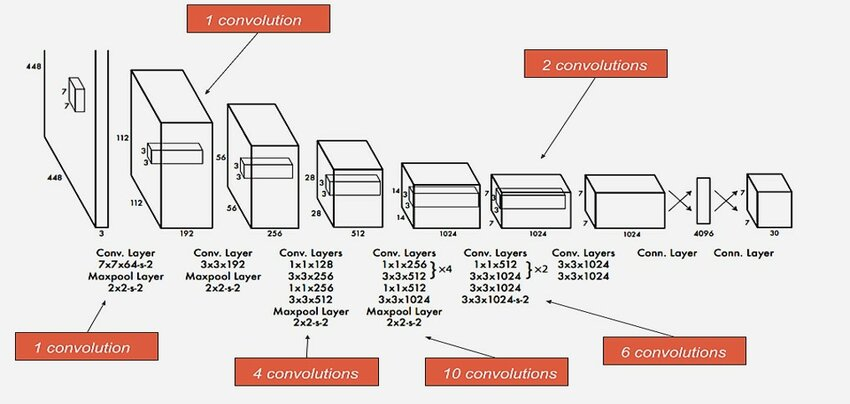
\includegraphics[width=0.95\textwidth]{logos/yolo_architecture.png}
        \caption{YOLO architecture overview}
        \label{fig:arch}
    \end{figure}
    
    Over the years, YOLO has evolved from its initial version to more advanced iterations like \textbf{\textcolor{black}{YOLOv4}}, each improving upon \textbf{\textcolor{black}{accuracy}}, handling of smaller objects, and \textbf{\textcolor{black}{inference speed}}. These advancements have made YOLO highly adaptable to diverse real-world applications, though it continues to face challenges such as maintaining performance in degraded image conditions like \textbf{\textcolor{black}{blur}}, \textbf{\textcolor{black}{noise}}, and \textbf{\textcolor{black}{occlusion}}.
\end{block}




\begin{block}{Challenges in Object Detection}
    \vspace{0.6cm} % Adds extra space between the "Challenges in Object Detection" title and content

    Despite its achievements, YOLO faces several persistent challenges that impact its performance in real-world scenarios. Key challenges include:

    \begin{itemize}
      \item \textbf{Multi-scale Training}: YOLO’s grid structure can struggle with objects of varying sizes. Multi-scale training helps to improve accuracy across small, medium, and large objects.

      \item \textbf{Small and Overlapping Objects}: Detecting small or overlapping objects is difficult due to limited pixel representation. Overlapping objects often lead to misclassification, requiring refined techniques for accuracy.

      \item \textbf{Low-Quality Images}: Factors like motion blur, noise, and occlusion degrade image quality, reducing detection accuracy. Enhancements are needed to make YOLO more robust under these conditions \cite{6}.
    \end{itemize}

    These challenges emphasize the need for ongoing research to enhance YOLO’s capabilities and ensure its reliability in diverse practical applications.
\end{block}

\begin{block}{Key Improvements in YOLO Versions}
    \vspace{0.6cm} % Adds extra space between the title and content

    YOLO’s evolution across versions has significantly enhanced its capabilities, addressing challenges such as detection accuracy, speed, and handling of small and overlapping objects. Below is a breakdown of the key advancements introduced in each version:

 \begin{figure}
    \centering
    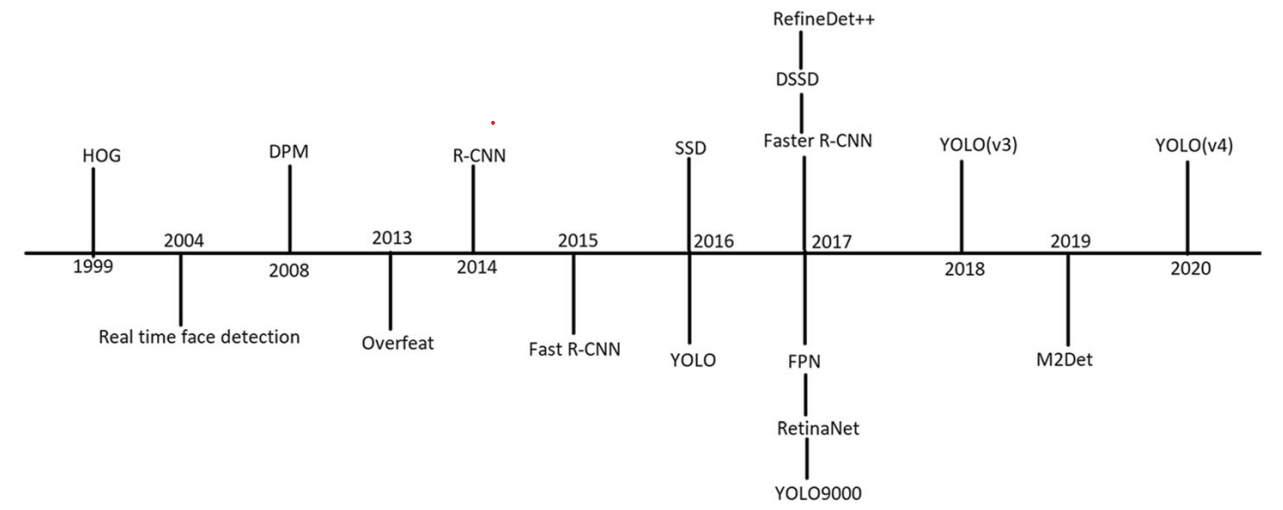
\includegraphics[width=0.95\textwidth]{logos/year.png}
    \caption{Figure 2: Year-wise Evolution}
    \label{fig:arch}
\end{figure}

\end{block}


\end{column}

\separatorcolumn

\begin{column}{\colwidth}


\begin{block}{YOLOv1}
    \begin{itemize}
      \item \textbf{Speed-Focused Architecture}: YOLOv1 introduced the concept of single-stage object detection, which processes the entire image in one pass, framing detection as a regression task instead of using multiple stages for classification and localization.
      \item \textbf{Grid-Based Detection}: YOLOv1 divides the image into a fixed grid, with each grid cell responsible for detecting objects. While this allowed for rapid predictions, the coarse grid led to limitations in detecting smaller objects and reduced localization accuracy.
    \end{itemize}
\end{block}

\begin{block}{YOLOv2}
    \begin{itemize}
      \item \textbf{Anchor Boxes for Flexible Detection}: YOLOv2 introduced anchor boxes, providing a way to detect objects of various shapes and sizes, making it more effective for real-world images with varied object scales.
      \item \textbf{Darknet-19 Backbone}: Replacing the earlier architecture, Darknet-19 allowed for deeper and more efficient feature extraction, while batch normalization stabilized training and increased detection performance.
      \item \textbf{High-Resolution Classifier}: YOLOv2 added a high-resolution classifier, improving detection accuracy by training the model at higher input resolutions, enhancing its ability to detect smaller objects.
    \end{itemize}
\end{block}

\begin{block}{YOLOv3}
    \begin{itemize}
      \item \textbf{Multi-Scale Predictions with Feature Pyramids}: YOLOv3 addressed small object detection by leveraging feature pyramids, enabling detection at different scales, which improved accuracy across object sizes.
      \item \textbf{Darknet-53 Backbone with Residual Connections}: This new backbone increased the model’s depth, allowing for better gradient flow and more detailed feature extraction, improving handling of complex, overlapping objects.
      \item \textbf{Sigmoid-Based Predictions for Class Confidence}: YOLOv3 utilized logistic regression for class predictions, simplifying the output and improving confidence scores for overlapping objects.
    \end{itemize}
\end{block}

\begin{block}{YOLOv4}
    \begin{itemize}
      \item \textbf{Cross-Stage Partial Networks (CSPNet)}: CSPNet was added to improve gradient flow and reduce computational complexity, allowing YOLOv4 to achieve higher accuracy with efficient resource usage.
      \item \textbf{Mosaic Data Augmentation}: This technique combined four images into one, creating a more varied training set that improved the model’s robustness across different object scales and positions.
      \item \textbf{Spatial Pyramid Pooling (SPP)}: SPP layers improved YOLOv4’s ability to detect objects at multiple scales by pooling at different levels, helping the model capture context around objects without impacting inference speed.
    \end{itemize}
\end{block}





\begin{block}{Experimental Setup}
    \vspace{0.5cm} % Adds extra space between the title and content
    
    Experiments utilized the widely-used MS COCO and PASCAL VOC datasets, selected for their diversity in object classes and environmental conditions, allowing for a robust evaluation of YOLO’s detection capabilities.

    Key degradation conditions were simulated to assess YOLO's robustness:

    \begin{itemize}
      \item \textbf{Blur:} Simulated motion or focus issues affecting object details.
      \item \textbf{Noise:} Replicated low-light or sensor noise that reduces clarity.
      \item \textbf{Rotation:} Tested detection of objects at varied orientations.
      \item \textbf{Cropping:} Assessed performance when objects are partially visible.
    \end{itemize}

    Training and evaluation were conducted on high-performance GPUs with images processed at different resolutions, highlighting YOLO’s adaptability and identifying areas for improvement.
\end{block}

\begin{center}
    \colorbox{lightblue}{%
        \begin{minipage}{0.95\textwidth} % Adjust the width as needed
            \vspace{1cm} % Add space at the top of the box
            \centering
            \textbf{Discover More Here!} \\[0.5cm] % Centered heading with some space below
            \vspace{1cm} % Add space above the QR code
            
\includegraphics[width=0.3\textwidth]{logos/VistaQR-website-github_com_rvk7021_DIP-poster-presentation-2.png} % Your QR code image path
            \vspace{1cm} % Add space below the QR code
        \end{minipage}
    }
    \vspace{2cm} % Add space below the QR code section
\end{center}


\end{column}

\separatorcolumn

\begin{column}{\colwidth}
    \begin{block}{Results and Discussion}
        \vspace{0.5cm} % Adds extra space between the title and content

    The model’s performance varied significantly with the type of image degradation applied during testing. The findings from our experiments indicate the following:

\begin{itemize}
      \item \textbf{Blur:} This condition resulted in an average precision decrease of 2.06%. This modest decline highlights the critical need for clarity in images, as blurriness can obscure important object details, leading to inaccuracies in detection. The model's ability to recognize features diminishes when images lack sharpness, emphasizing the importance of employing effective stabilization and focus techniques in real-world applications.

      \item \textbf{Noise:} The introduction of noise to the images led to a more substantial drop in performance, with average precision lowered by 12.01%. This significant decline suggests that noise, particularly in low-light conditions, can severely impact the model's capability to accurately identify and classify objects. It points to the necessity for incorporating robust noise reduction techniques or advanced preprocessing methods to mitigate the effects of noise and improve detection accuracy.

      \item \textbf{Rotation:} Accuracy diminished by 24.23% under rotated conditions, underscoring the challenges posed by non-standard object orientations. The model's difficulty in recognizing objects at various angles suggests that additional strategies, such as augmenting the training dataset with rotated images, could enhance the model's robustness against orientation variations and improve its generalization capabilities in practical scenarios.
\end{itemize}

    \begin{figure}
    \centering
    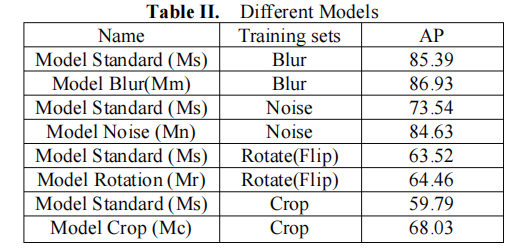
\includegraphics[width=0.95\textwidth]{logos/res_poster.png}
    \caption{Model accuracy under different degradations}
    \label{fig:results}
  \end{figure}
  
    Importantly, training the model on datasets that include a variety of degradation conditions has shown to improve robustness. Exposure to challenging scenarios during the training phase equips the model with the necessary features to handle similar difficulties during inference. This finding demonstrates the value of data augmentation and diverse training methodologies in developing resilient object detection models that can perform reliably in real-world environments \cite{7}.
  \end{block}

  \begin{figure}
    \centering
    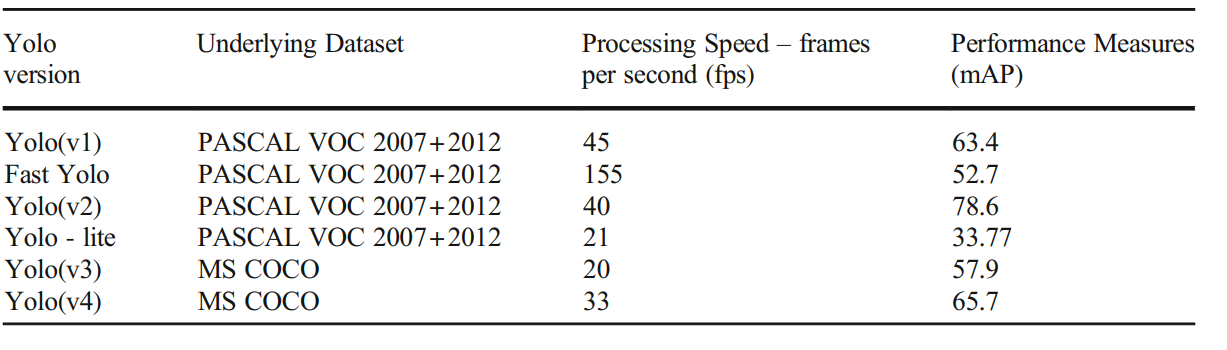
\includegraphics[width=0.95\textwidth]{logos/yolo.png}
    \caption{Model accuracy under different degradations}
    \label{fig:results}
  \end{figure}
  
\begin{block}{Conclusions}
    \vspace{0.5cm} % Adds space between the title and content
    
    In conclusion, YOLO remains one of the most effective object detection algorithms in computer vision, primarily due to its exceptional \textbf{speed} and \textbf{efficiency}. Its single-stage architecture allows for real-time processing, making it particularly suitable for applications in areas such as \textbf{autonomous driving}, \textbf{video surveillance}, and \textbf{robotics}.

    However, challenges remain in scenarios involving degraded images—such as those affected by \textbf{blur}, \textbf{noise}, or \textbf{occlusion}—and in detecting \textbf{small and overlapping objects}. Future work will focus on enhancing YOLO’s capability to improve detection accuracy in \textbf{poor-quality images} and ensure its continued relevance in practical applications.
\end{block}

\begin{block}{Acknowledgments}
    \vspace{0.5cm} % Adds extra space between the title and content
    
    We sincerely thank \textbf{Dr. Tapan Kumar Jain} for his valuable insights and guidance throughout this project. We also extend our gratitude to the \textbf{Dean} and \textbf{Director of IIIT Nagpur} for their support and encouragement, which made this work possible.
\end{block}

\begin{block}{References}
    \vspace{0.5cm} % Adds space between the title and content
    \begin{thebibliography}{99} % Use {99} to allow for up to 99 references
        \bibitem{Diwan2023} 
        T. Diwan, G. Anirudh, and J. V. Tembhurne, 
        ``Object detection using YOLO: challenges, architectural successors, datasets and applications,''
        \textit{Journal Name, Volume}(Year), pages. 

        \bibitem{Liu2023} 
        C. Liu, Y. Tao, J. Liang, K. Li, and Y. Chen, 
        ``Object Detection Based on YOLO Network,''
        \textit{Journal Name, Volume}(Year), pages.
    \end{thebibliography}
\end{block}

  
\end{column}

\separatorcolumn
\end{columns}
\end{frame}
\end{document}
